\documentclass{hertieteaching}
%\usepackage{cancel}
%\usepackage{hyperref}
%
\title{Topic models: evaluation}

\begin{document}

\maketitle

\begin{frame}{Plan}

\begin{itemize}
  \item Evaluation
  \item Statistical model evaluation
  \item Human model evaluation
  \item Statistical topic evaluation
  \item Human topic evaluation
  \item Case study
\end{itemize}


\end{frame}

\begin{frame}{Evaluation}

There are two main modes of evaluation:
\begin{itemize}
  \item Statistical
  \item Human / substantive
\end{itemize}
and two natural levels
\begin{itemize}
  \item The models as a whole
  \item The topics it creates
\end{itemize}

\bigskip
Overall message: These are not yet well aligned
\begin{itemize}
  \item We will emphasize substance and topics 
\end{itemize}




\end{frame}

\begin{frame}{Held-out likelihood}

Since documents are assumed to be bags of words, then we can
\begin{itemize}
  \item set aside some proportion of each document
  \item fit a topic model to the remainder
  \item ask how probable the held out parts are under the model
\end{itemize}
The \textsf{stm} package calls this `heldout likelihood by document completion'
\begin{itemize}
  \item Returns the average log probability of the heldout documents' words
\end{itemize}

\end{frame}



\begin{frame}{Choice of k}


\centerline{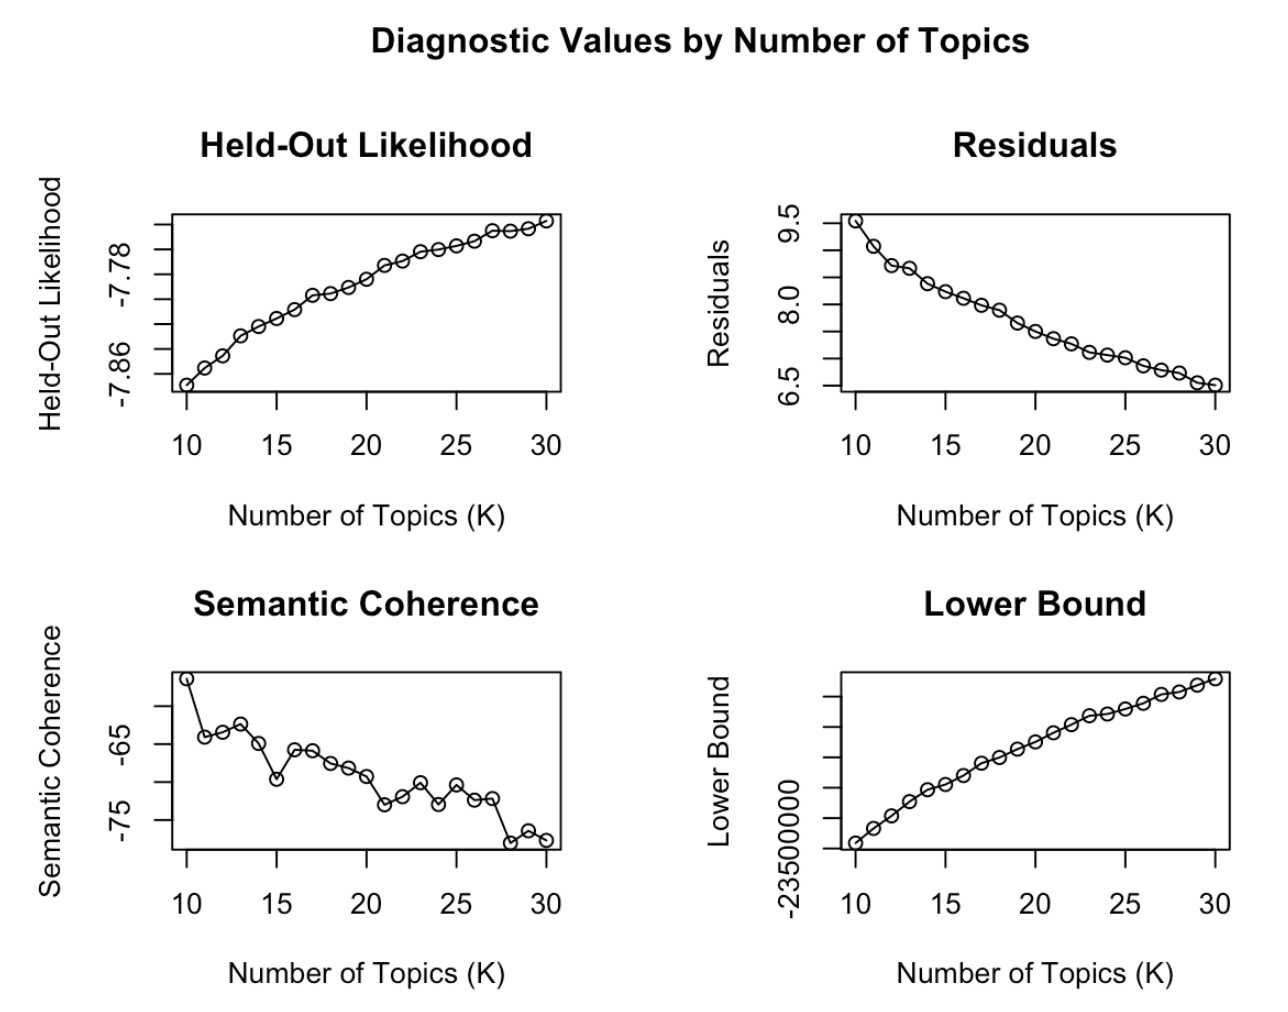
\includegraphics[scale=0.4]{pictures/heldout-lda}}

\end{frame}

\begin{frame}{Construct validity}

\centerline{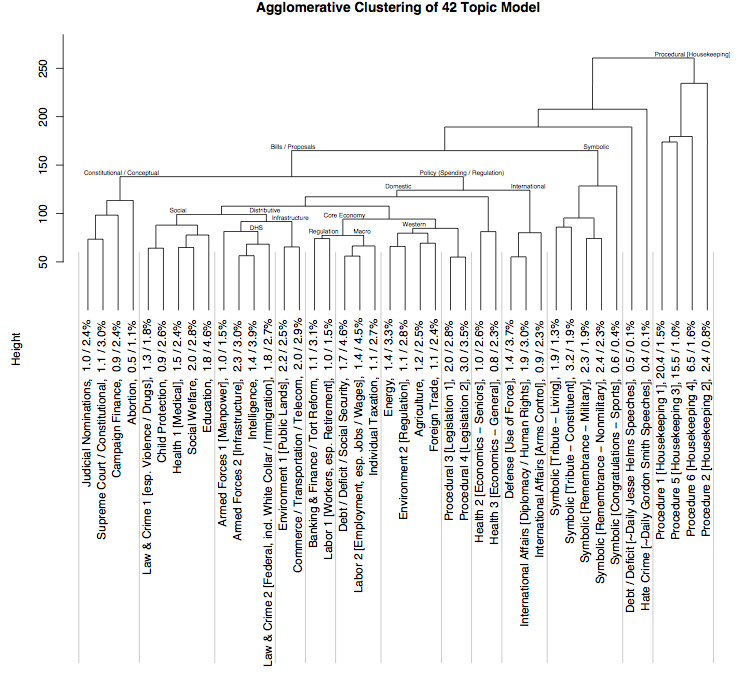
\includegraphics[scale=0.4]{pictures/topic-clustering}}

\end{frame}


\begin{frame}{Choice of k}

\medskip
\begin{quote}
The results presented in this paper ... assume there are 43 
topics present in the data. I varied the number of assumed topics
from only five topics, up to 85 different topics. Assuming too few
topics resulted in distinct issues being lumped together, whereas 
too many topics results in several clusters referring to the same
issues. During my tests, 43 issues represented a decent middle
ground. \\
\hfill\parencite{Grimmer2010} 
\end{quote}

\pause

We can be realists or anti-realists about topics
\begin{itemize}
  \item Anti-realism: topics are `lenses'
  \item Realism: topics are real discourse units, e.g. themes, categories, etc.
\end{itemize}

\pause

We can \textit{try} to be realists about the conditional independence assumption
\begin{itemize}
  \item Once we know the topic indicator, remaining word variation is just random $\rightarrow$ unpredictable
\end{itemize}
That's seldom true for mundane linguistic reasons

\end{frame}








%\begin{frame}{Prediction}
%
%For truly out of sample documents
%
%Prediction is a little more involved for a 
%\textsf{fitNewDocuments} and \textsf{alignCorpus}
%  
%\end{frame}
%


\begin{frame}{Topic coherence, exclusivity, and frex}

\textsc{Semantic coherence}

\begin{itemize}
  \item Regularly co-occurring words should be in  topics together
\end{itemize}

\textsc{Exclusivity}

\begin{itemize}
  \item High precision words make for \textit{well-separated} topics
\end{itemize}
$$
\frac{\beta_w^{(j)}}{\sum_{k\neq j} \beta_w^{(k)}}
$$

\textsc{frex}
\begin{itemize}
  \item A weighted average of exclusivity and simple frequency, favouring exclusivity
\end{itemize}


\medskip
These are heuristic measures, so don't take them too seriously.

\end{frame}

\begin{frame}{Humans in the loop}

Experiments by \textcite{Chang.etal2009} using
\begin{itemize}
  \item word intrusion: ``which of the following words does not belong?''
  \item topic intrusion: ``which of these topics do not make sense for this passage?''
\end{itemize}

Unfortunately, these are measures that covary \textit{negatively} with the previous statistical measures

\end{frame}

\begin{frame}{Chang et al. 2009}

\centerline{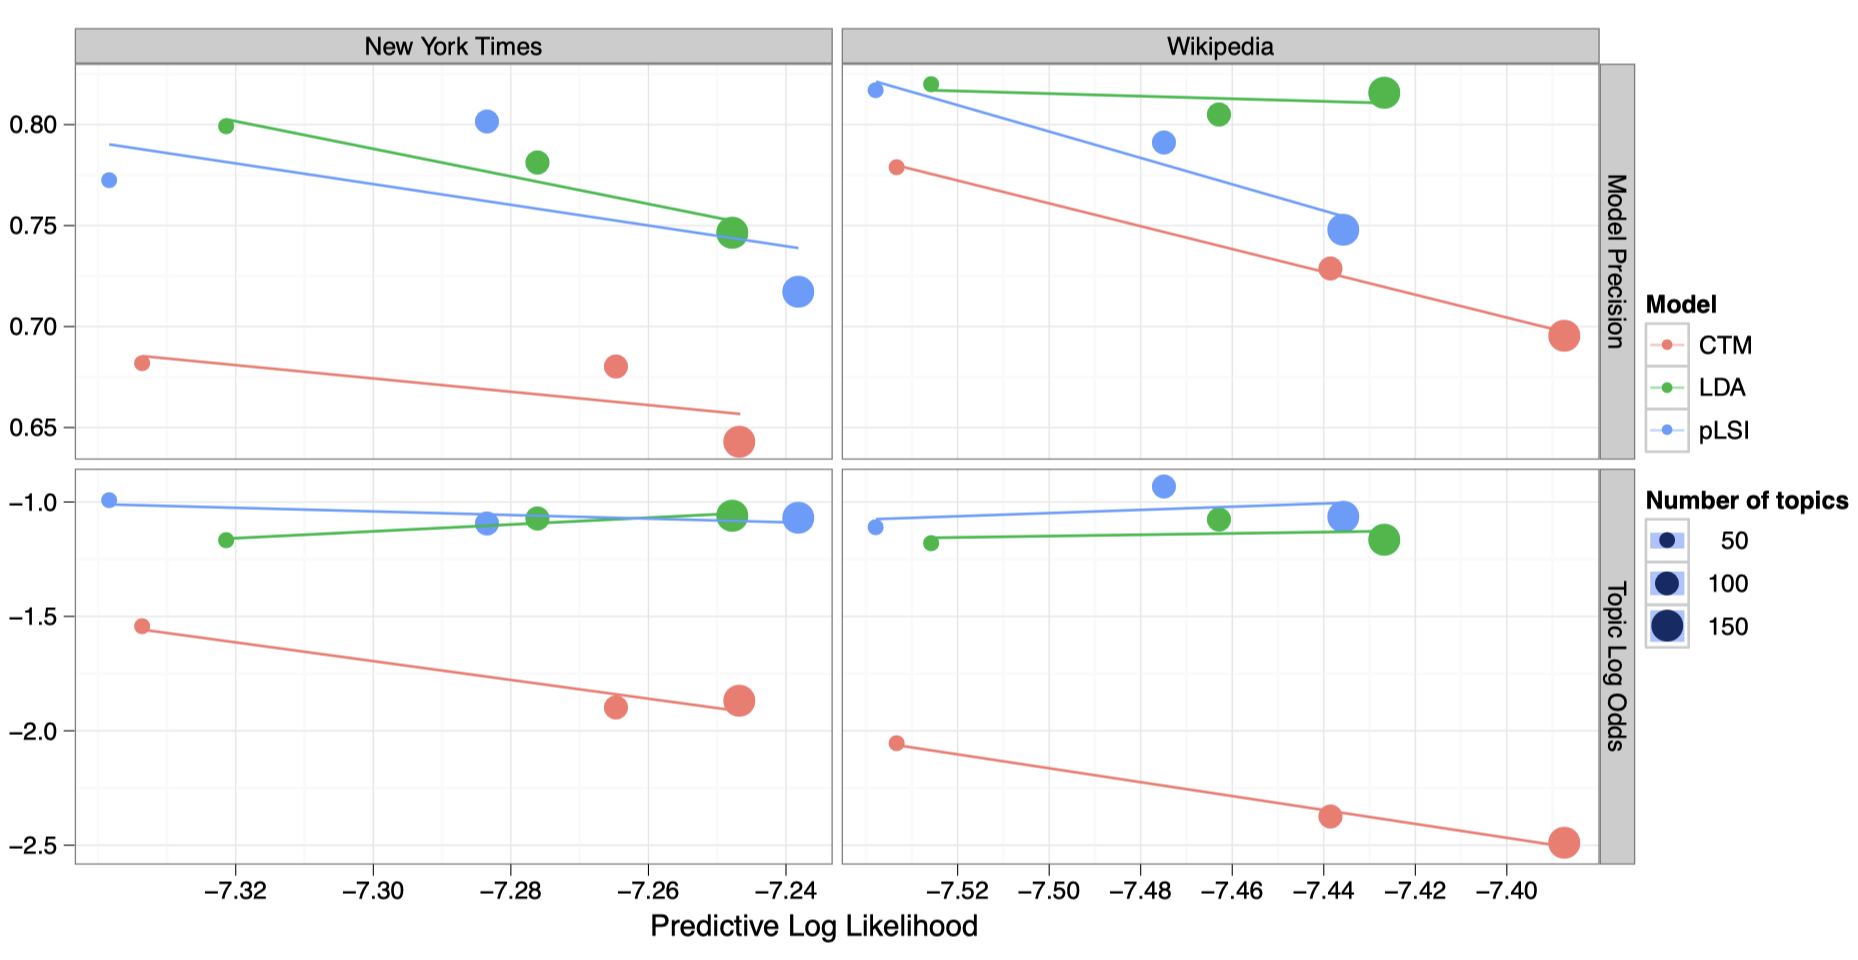
\includegraphics[scale=0.4]{pictures/chang2009}}

\end{frame}


\begin{frame}{Gamson and Modigliani redux}

\centerline{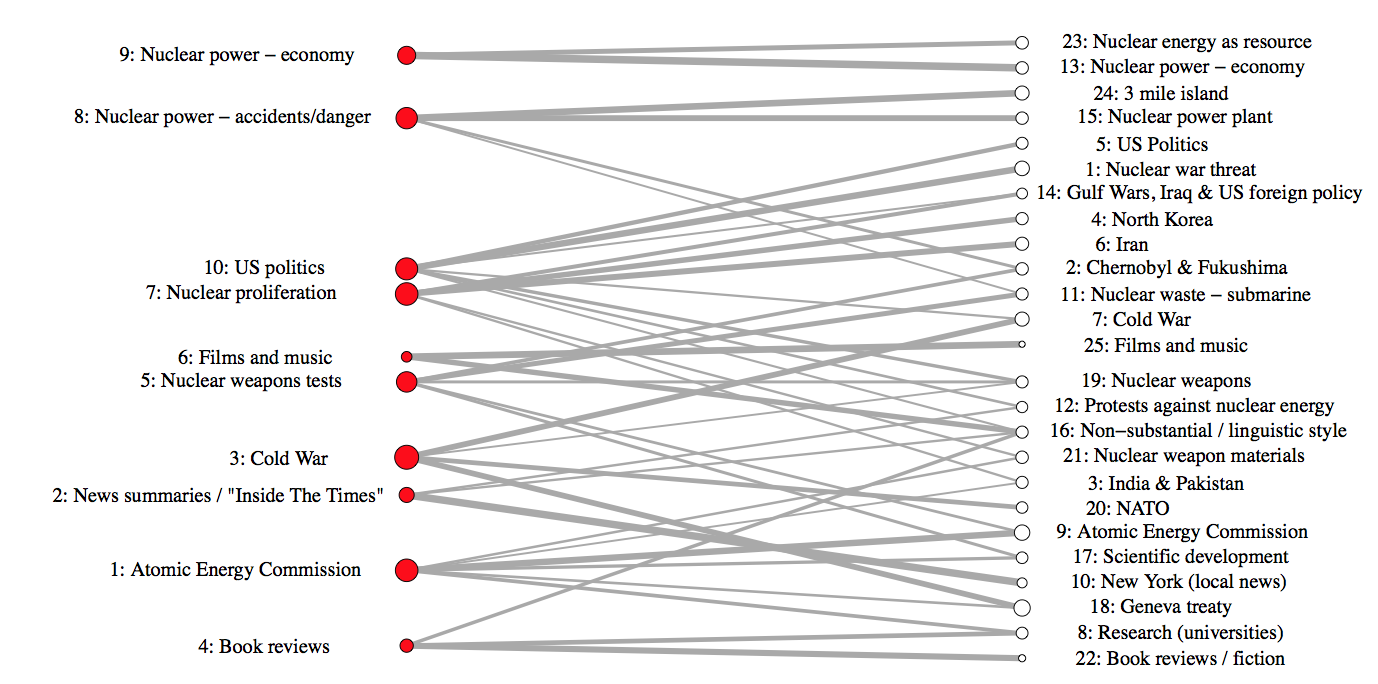
\includegraphics[scale=0.45]{pictures/nested-topics-nuclear}}

from van Atteveldt et al. (MS)


\end{frame}

\begin{frame}{Case study}

The real timeline of \textcite{Baerg.Lowe2020}

\begin{itemize}
  \item Paper and basic results sent to ACL conference workshop (wins prize)
  \item Conference paper expanded to political science length journal article and sent out to review
  \item (repeat several times)
  \item Reviewers do not believe topics measure what we say they measure
  \item Embark on a manual validation exercise (random kwics etc.)
  \item \ldots
  \item Publish
\end{itemize}

Disagreements were all about measurement validity.

Nobody ever asked for the heldout log likelihood, coherence, exclusivity, or choice of $K$.

\end{frame}

\begin{frame}{Evaluation}

Recommendations if you feel the need to topic model:
\begin{itemize}
  \item Don't take the statistical evaluation measures very seriously
  \item Work at getting interpretable substance right
  \item Take what you need from the model (we threw away some topics and aggregated some others) 
  \item You can always fit on a random sample and apply to the remainder of your documents
  \item Your idea of a topic is hard to communicate, even to your friends, so don't expect any machinery to intuit it
  \item Make sure it all replicates!
\end{itemize}

\end{frame}



%
%## Explaining topic prevalence: A case study
%
%Catalinac (2016) Examines the effect of electoral reform
%
%- Before 1994: SNTV-MMD (more intraparty competition)
%- After 1994: Mixed member majoritarian (PR + SMD)
%
%LDA on N = 7497 candidate manifestos for Diet 1950-2009
%
%- Hand transcribed, OCR failed
%- Things are complicated in Japanese!
%
%Characterizing campaigns across 50+ years
%
%- What do candidates talk about?
%- How did electoral reform change incentives?
%- Why increasing interest in military foreign action?
%
%## Japanese Manifestos
%
%```{r, out.width = '95%'}
%knitr::include_graphics("pictures/jpmanifesto.png")
%```
%
%## Japanese Manifesto Topics
%
%```{r, out.width = '110%'}
%knitr::include_graphics("pictures/jptopic.png")
%```
%
%## Manifesto Content over Time
%
%```{r, out.width = '70%'}
%knitr::include_graphics("pictures/jpcontent.png")
%```
%
%## Foreign Policy Content
%
%```{r, out.width = '60%'}
%knitr::include_graphics("pictures/jpforeign.png")
%```
%
%## Doing it all at once
%
%Structural topic model [@Roberts.etal2014].
%
%```{r, out.width = '80%'}
%knitr::include_graphics("pictures/lda-stm2.pdf")
%```
%
%## Doing it all at once
%
%```{r, out.width = '90%', fig.cap = "(Nielsen 2013)"}
%knitr::include_graphics("pictures/nielsen-stm.png")
%```
%
%## Doing it all at once
%
%```{r, out.width = '90%', fig.cap = "(Nielsen 2013)"}
%knitr::include_graphics("pictures/nielsen-two-props.png")
%```
%
%## Practical issues: Baerg and Lowe
%
%A timeline:
%
%- Paper and basic results sent to ACL workshop (wins prize)
%- Inflated to poli-sci length paper and sent to review
%- Reviewers do not believe topics measure what we say they measure
%- We validate manually, and compare to other measures
%- Reviewers do not believe topics measure what we say they measure
%- We validate manually, and compare to other measures
%- (repeat)
%
%Publish.
%
%Disagreements were *all* about measurement
%
%##
%
%```{r, out.width = '90%'}
%knitr::include_graphics("pictures/filedrawer.jpg")
%```
%




\begin{frame}[allowframebreaks]
\frametitle{References}
\printbibliography	
\end{frame}

\end{document}
